%----------------------------------- Context ----------------------------------%
%-- Why biometric
Whether it is for security or economical reasons, recognizing individuals is a problem that has always demanded innovation in order to create systems that are robust and user friendly.
Biometrics is essentially a pattern recognition problem in which an individual's identity is assessed by using a specific biometric trait, or a combination of several traits, directly possessed by the user.
Biometric systems seek to recognize individuals using physiological or behavioral characteristics such as face, finger print, iris, signature, gait, or voice (\cite{jain06}).
Unlike other current identification methods (\emph{e.g.}, passwords, access cards and identification numbers and cards), these characteristics are unique to each individual and cannot be lost, stolen or easily reproduced.
Therefore, they can be used to prevent theft and fraud.
In a globalization context, where individuals move more and more across borders, such types of recognition systems are particularly interesting as they facilitate mobility as well as maintain an acceptable level of security.

There are three types of applications in biometric recognition -- verification, identification, and surveillance (\cite{jain06}).
In verification applications, an individual enrolled in the system identifies himself and provides a biometric sample.
The biometric system then seeks to verify that the sample corresponds to the model of that specific individual.
In contrast, in identification applications, an individual provides a biometric sample, and the system seeks to determine if the sample corresponds to the model of any of the individuals registered in the system.
Surveillance applications differ slightly from identification applications in that the sampling process is performed discretely in an unconstrained scene.
It then seeks to determine if a given biometric sample corresponds to the model of a restrained list of individuals under surveillance, \emph{e.g.}, screening for criminals or terrorists in an airport setting.

%-- Why face recognition
Over the past decade, face recognition has received considerable attention in the area of biometrics due to the wide range of commercial and law enforcement applications, as well as the availability of affordable technologies.
Recognizing individuals in video streams is relevant in different scenarios and applications.
One is closed-set identification or verification for access control applications, where individuals enrolled in a system must either be solely identified with face images prior to accessing secured resources, or have their identity verified after having used other identification means (password, key card, etc.).
Since face recognition does not require the cooperation of individuals involved in the recognition process, considerable advantage over other biometric modalities (\cite{jain05, zhao03}).
It can thus also be used for open-set video surveillance in unconstrained scenes, where individuals enrolled to a watch list must be recognized among other people unknown to the system.
Practical applications includes: identification at access control points, and user verification of mobile devices such as laptop or cell phone, and surveillance for screening criminals or terrorists in dense and moving crowds at major events and airports.

Several methods to recognize faces in static images are described in \cite{jain05, zhang09,zhao03}.
However, due to the presence of intra-class variations when acquiring images from unconstrained scenes (\emph{e.g.}, illumination, pose, facial expression, orientation and occlusion), their performance may degrade considerably in video sequences. 
Still, the first attempts to recognize faces in video streams consist in applying extensions of static images techniques (\cite{matta09}).
This way, one of the more basic techniques for image-based face recognition, Eigenfaces (\cite{turk91}), has been adapted for video by introducing a similarity measure for matching video data (\cite{maeda99, satoh00}).
The similarity between distinct sequences is determined by the smallest distance between frame pairs (one from each video) projected in different subspaces. 
In the same fashion, an extension of Fisherfaces (\cite{belhumeur97}) was obtained by adapting this similarity measure (\cite{satoh00}).
Active appearance models, a statistical model of the face that combines shape and intensity, was modified by separating the inter-class variability from the intra-class one (\cite{edwards99}) and by developing a multiview dynamic facial model to extract normalized facial textures (\cite{li01_face}).
Finally, Elastic Bunch Graph Matching (\cite{wiskott97}) was incorporated in a complete video-based face recognition system (\cite{steffens98}).

Other general pattern recognition techniques have also been adapted to video-based face recognition problems.
For instance, used in conjunction with a confidence measure to filter video frames suitable for classification, radial basis function neural networks have been modify to train over sequences, rather than individual frames (\cite{koh02, balasubramanian09}).
Hierarchical discriminative regression trees (\cite{hwang00}) have been applied directly to face recognition by considering video sequences only as a source of data were frames are used independently (\cite{weng00}).
Unsupervised pairewise clustering has also been developed to built a graph structure that chains together similar views in video sequences (\cite{raytchev03}).

To further reduce matching ambiguity, face recognition applications specifically designed for video sequences combine spatial and temporal information contained in video streams.
Head and facial motion during the sequence can be exploited by either estimating the optical flow or tracking a few facial landmarks over time with a template matching strategy (\cite{chen01}).
Temporal dynamics and statistics of training video sequences can also be modeled with a Hidden Markov Model, particle filtering, or time series state space models (\cite{hadid04, li01, liu03, zhou03}).
Instead of directly exploiting temporal information of each successive frame in a video sequence, a probabilistic appearance manifold approach can also be used.
Bayesian inference is then used to include temporal coherence in distance calculation when performing recognition (\cite{cevikalp10, lee05, wang08}).
Although they were not design to exploit temporal informations, other authors address problems that are specific to unconstrained scenes during video-based face recognition, such as change in the illumination conditions (\cite{arandjelovic09, wang10}).

%--------------------------- Face recognition system --------------------------%
\begin{figure*}[t] \centering
  \fbox{
  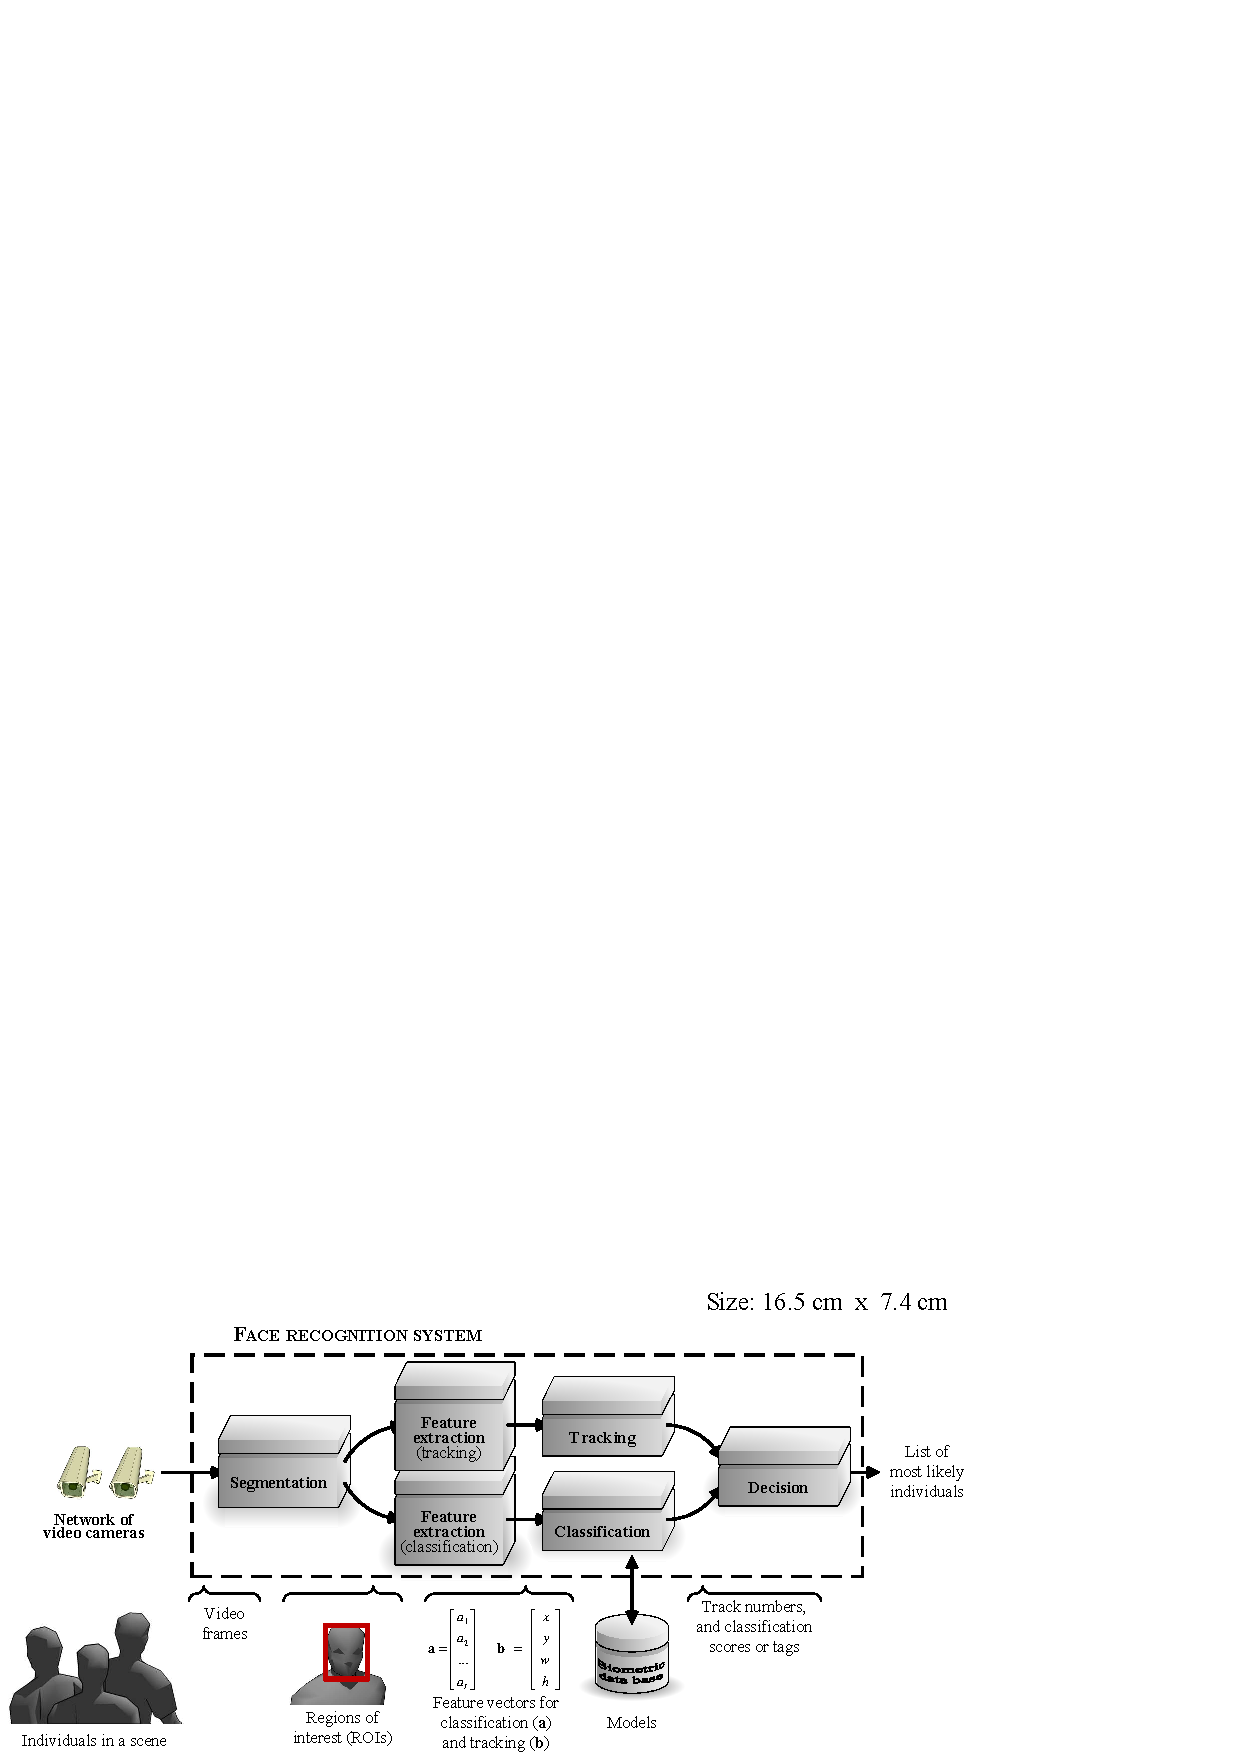
\includegraphics[width =0.97\linewidth, viewport= 0cm 0cm 16.5cm 7.4cm, clip]
 		              {c3_fig2} }
  \caption{A generic track-and-classify biometric system for video-based face recognition}
	\label{fig:c0_faceRec}
\end{figure*}
%-------------------------- /Face recognition system --------------------------%

In this thesis, video-based face recognition is performed with a track-and-classify system that combines the responses of a classifier to kinematic information of individuals and the appearance of faces in a scene (see Figure \ref{fig:c0_faceRec}).
It is assumed that 2D images in the video streams of an external 3D scene are captured using one or more IP or network cameras.
Each camera captures a sequence of 2D images, or frames, from the external scene, and each frame provides the system with a particular view of individuals populating the scene.

First, the system performs segmentation to locate and isolate regions of interest (ROIs) corresponding to the faces in a frame.
In this thesis, the well known Viola-Jones face detection algorithm (\cite{viola01}) is used for this task.
From the ROIs, features are extracted for tracking and classification.
The tracking features can be the position in the 2D images, speed, acceleration, and track number assigned to each ROI on the scene so that the tracking module may follow the movement or expression of faces across the frames.
On the other hand, classifiers will require invariant and discriminating classification features extracted from the ROIs, so that the classification module may match input feature patterns to an individual registered in the system.
Facial matching may be implemented with templates, statistical, or neural pattern classifiers.
Since feature-based methods like Elastic Bunch Graph Matching tend to become complex when several individuals and cameras are involved, the predominant techniques used with this type of architecture are the same appearance-based methods (Eigenfaces, Fisherfaces, etc.) used to represent faces in static 2D images (\cite{zhang09, zhao03}).

The decision module may then combine and accumulate the responses from the tracking and classification modules over several frames (\cite{granger01}).
With identification and surveillance applications for instance, ambiguity is reduced by accumulating responses (classification scores) obtained for each frame over the trajectory of each individual in the scene.

This thesis discusses the use of a video face recognition for closed-set identification, in applications such as access control for security checkpoints or for computer login.
More specifically, it is interested in the process by which facial models of individuals are updated over time with new data in the face recognition system. 
It explores the two most plausible scenarios that can occur in this situation: (1) new individuals are presented one at a time to build the models (enrollment), or (2) individuals already seen by the system are presented, again, one at a time, to update the existing models (re-enrollment).  
It is assumed that new labeled reference data becomes available over multiple (re)enrollment sessions, or when operational scenarios are analyzed off-line, and may belong to new individuals to be registered in the face recognition system.
While the design and update of the class models can be performed off-line, identification, among several individuals registered in the face recognition system, of the ROI(s) in each in a frame must be performed in real time.

%------------------------------ Problem statement -----------------------------%
\section{Problem Statement}

\subsection{Biometric Systems}

%-- Why neural network classifiers
%-- Biometric / face recognition -- lack of data
In biometric applications, including face recognition, matching is typically performed by comparing query samples captured with some sensors against biometric class models (\emph{i.e.}, an individual's facial model) designed with reference samples captured during an enrollment process.
In its most basic form, a biometric model consists of a set of one or more templates (features representing a person's biometric trait) stored in a biometric data base (Figure \ref{fig:c0_faceRec}).
Since reference data is sampled from an unknown probability distribution, biometric class models may also consist of a statistical representation estimated by training a discriminative classifier on these data to improve robustness and reduce resources.
Then, neural or statistical classifiers implicitly define the biometric model of an individual's physiological or behavioral trait with a set of parameters and map the finite set of reference samples defined in an input feature space to a set of predefined class labels in an output space.
The collection and analysis of reference data are often expensive and time consuming because real individuals are involved in the process.
Therefore, classifiers are often designed using some prior knowledge of the underlying data distributions, a set of user-defined hyperparameters (\emph{e.g.}, learning rate), and a limited amount of reference data.

%-- Why adaptation 
In real applications, it is possible to acquire new reference samples at some point in time, after a classifier has originally been trained and deployed for operations.
Labeled and unlabelled reference data can be acquired to update the class models of pre-existing individuals through re-enrollment sessions and analysis of operational data, or enrollment of new individuals in the system.
In addition to changes that may occur when acquiring images from unconstrained scenes, the physiology of individuals may change over time, either temporarily (\emph{e.g.}, haircut, glasses, etc.) or permanently (\emph{e.g.}, scars, aging).
New information such as input features and new individuals may emerge, and previously acquired data may become obsolete in dynamically changing classification environments (\cite{granger01, tsymbal08}).

%-- Adaptive biometric systems - templates
In the literature, specialized adaptive biometric systems have been proposed to define and refine biometric models according to intra-class variations in new reference samples.
These methods focus on procedures to update templates initially designed during enrollment, and perform recognition with a biometric model consisting of one, several, or even a super template (several templates combined to form a single one).
The update procedures either involve semi-supervised learning strategies with highly confident unlabeled data obtained during operations (\cite{poh09, rattani10}), clustering and editing techniques to update selection of user templates from a gallery with labeled reference samples (\cite{uludag04}), or on-line learning of genuine samples over time to update each user's single super template (\cite{jiang02}).
These methods have been showed to be vulnerable to intra-class variations, such as outliers, dispersion and overlap in class distributions.
In all cases, the biometric facial model of an individual tends to diverge from its underlying class distribution due to limited reference data, complexity, and changes in the classification environments.

\subsection{Statistical and Neural Classifiers}

Although using statistical and neural pattern classifiers may represent a flexible solution to a biometric recognition problem, their performance depends heavily on the availability of representative reference data.
Moreover, the majority of the classifiers proposed in the literature assume a static classification environment and can only perform \emph{supervised batch learning} of a finite data set.
To account for new information from new data, they must accumulate it in memory and train from the start using all previously acquired learning data.
Otherwise, new data may corrupt the classifier's previously acquired knowledge, and compromise its ability to achieve a high level of generalization during future operations (catastrophic forgetting problem).
In the context of a face recognition problem, this would lead to the corruption of facial class models when new data are added in time.

Video-based face recognition is becoming an important function in enhanced surveillance systems, which must simultaneously process many video feeds.
As these applications must perform in real-time, the design of efficient systems for facial matching involves a trade-off between classification speed, accuracy, and resources for the storage of facial models.
For instance, today's video surveillance networks are comprised of a growing number of IP cameras.
The need to design and store representative facial models for recognition -- either more user templates or their statistical representation -- increases the resource requirements of the system.
In addition, matching captured facial images to models for a large number of frames from different sources may severely increase the computational burden.
Finally, the memory and time complexity associated with storing and relearning from the start on all cumulative data makes supervised batch learning impossible in this situation. 

%-- Incremental learning
When new data becomes available, classifiers can be updated through \emph{supervised incremental learning} in order to accommodate new knowledge and avoid a growing divergence between class models and their underlying distributions. This method does not involve the redundant and costly computations of batch learning; it rather reduces the memory resources associated with storing classifiers.

Learning and adapting classifiers in changing classification environments raises the so-called stability-plasticity dilemma, where stability refers to retaining existing and relevant knowledge while plasticity enables learning new knowledge (\cite{grossberg88}).
The literature proposes many classifiers which re-estimate their own parameters and architecture through incremental learning (\cite{carpenter91, chakraborty03, fritzke96, okamoto03, ruping01}).
However, if the plasticity of these classifiers is not adjusted to accommodate new knowledge presented with new reference data, they can still be affected by the catastrophic forgetfulness problem (\cite{canuto00, dubrawski97, fung03, granger07, kapp09}).

\subsection{Adaptive Ensembles}

Recently, various methods employing adaptive ensembles of classifiers to perform incremental learning have been put in practice (\cite{polikar01, kapp10}).
For a wide range of applications, where adaptation is not necessarily required, classifier ensembles allow to exploit several views of a same problem to improve the overall accuracy and reliability.
With the use of a combination function, they also offer a flexibility over single classifiers in how class models can be managed and adapted. 
These methods can be divided in three general categories (\cite{kuncheva04}).
Dynamic combination, or ``horse racing'', methods where individual base classifiers are trained in advance to form a fixed ensemble where only the combination rules is changed dynamically (\cite{blum97, widmer96, xingquan04}).
Methods that rely on new data to update the parameters of ensemble base classifiers an online learner (\cite{gama04}).
If blocks of data are available, training can also be performed in batch mode while changing or not the the combination rule at the same time (\cite{breiman99, ganti02, oza01, wang03}).
The last main category consists of methods that grow ensembles by adding new base classifiers and replacing old or underperforming ones when new data is available (\cite{chen01, street01, kolter07, tsymbal08}).
Finally there are adaptive ensembles that use hybrid approaches that combine adding new base classifiers and adjusting the combination rule to update class models.
The most notable are streaming random forests with entropy (\cite{abdulsalam11}), Hoeffding tree with Kalman filter-based active change detection using adaptive sliding window (\cite{bifet10}), maintaining and choosing the better of two ensembles trained with current and old data (\cite{scholz06}), and the AdaBoost-like Learn++ (\cite{polikar01}).

Among these methods, horse racing approaches cannot accommodate new knowledge since base classifiers in the ensemble are never updated with new data.
On the other hand, while online learners and growing ensembles can be used to explore unknown regions of the feature space, most methods focus on the notion of concept drift where underlying class distributions changes in time.
They incrementally append new classifiers to a pool without updating pre-existing members to change their parameters and risk losing old knowledge.
While these classifiers are trained with new data, their plasticity (or learning dynamics) is set beforehand and remains fixed throughout the learning process, without being adjusted to accommodate new knowledge.
Their claim is that old concepts, represented by old data should never be revisited and \emph{reinforced} in contrast with new concept presented with new data.
Although this may happen in a face recognition application, when classes are added and removed from the system for instance, it is not necessarily the case.
In fact, when few biometric reference samples are available, the change that most commonly occurs is the knowledge of the underlying distributions, which is initially incomplete.
Moreover, face recognition systems in unconstrained scenes are often faced with recurring changes regarding the environment (\emph{e.g.}, light effect over the course of a day) and the individuals to recognize (beard, haircut, glasses, etc.).
In this context, adaptive ensemble methods that focus on concept drift may then forget old concepts that are still valid.

As it is detailed with the Learn++ algorithm (\cite{polikar01}) in Appendix \ref{sec:c0_learn++}, methods that rely exclusively on adding new ensemble members to explore the feature space become problematic if all classes are not always represented.
With the current face recognition application for instance, when new data becomes available after a classifier is designed and deployed in the field, it will most likely be sampled from few, or even, one person at a time. 
While previously trained classifiers will not be able to recognize new classes, the ones trained with the new data will contained only the facial models of individuals registered in the system at that time.

%-------------------------- Objectives & contribution -------------------------%
\section{Objective and contributions}

This thesis addresses the challenges mentioned before and seeks to provide a video face recognition system with a mean to perform enrollment and update of biometric models \emph{incrementally} when new data becomes available.
In the context of real-world video applications, where classifier predictions must be accurate and be available in real-time, an ideal face classifier must accommodate emerging reference samples such that  two objectives are minimized: classification error rate and computational cost.
To achieve this, the relationship between a classification environment, where a classifier's decision boundaries are defined, and an optimization environment, comprise of a hyperparameter search space and an objective space, is studied and characterized.
The result, and the core of this thesis, is a supervised incremental learning strategy based on particle swarm optimization (PSO) that is used to evolve a swarm of fuzzy ARTMAP (FAM) neural networks in response to new data.
As each particle in a hyperparameter search space corresponds to a FAM network, the learning strategy co-optimizes all classifier parameters -- hyperparameters, weights, and architecture -- in order to maximize accuracy, while minimizing computational cost and memory resources.

In addition to the incremental learning strategy, this thesis presents the following key contributions.
\begin{itemize}
	%-- Incremental learning properties
	\item The original definition of incremental learning is reconsidered.
The original definition, proposed by (\cite{polikar01}), states a classifier that can perform supervised incremental learning should:
\begin{enumerate}
	\item allow learning of additional information from new data, 
	\item not require access to the previous learning data,
	\item preserve previously acquired knowledge, and
	\item accommodate new classes that may be introduced with the new data.
\end{enumerate}
In order to mitigate corruption of previous knowledge when learning new data, a fifth property is considered: the classifier should also adapt its plasticity by adjusting its hyperparameters for accurate and timely recognition.
Furthermore, the second property is changed so that some previously acquired knowledge is necessary during the incremental learning process.
Otherwise, adaptation is only performed according to new data, and the classifier is subject to the problem of catastrophic forgetfulness.
	%-- Dynamic optimization problem
	\item Adapting FAM's plasticity by adjusting its hyperparameters with a particle swarm optimization (PSO) algorithm during incremental learning in order to maximize accuracy is shown to be a dynamic optimization problem.
More specifically, it is shown to correspond to a type III dynamic optimization problem, where both the location of the optimum on the objective function, as well as its value, change in time.
To properly adapt FAM networks to new data, dynamic particle swarm optimization (DPSO) must be use, otherwise performance decreases during the learning process.  
	%-- Correlation between particle and classifier diversity
	\item It is empirically shown that genotype diversity in the hyperparameter search space is correlated with classifier diversity in the classification environment.
When a pool of FAM classifiers are trained on the same data, the resulting decision boundaries of each FAM network change according the hyperparameter values with which it was trained.
With several correlation and diversity indicators, results then indicate that, as genotype diversity among swarm of particles (\emph{i.e.}, hyperparameter values) increases, diversity among a corresponding  pool of classifiers also increases.
This property allows the diversity of solutions to be easily controlled in the optimization environment.
	%-- Ensemble selection
	\item Following the previous contribution, a greedy search algorithm is presented to perform an efficient selection of diversified ensembles of classifiers among a pool.
Instead of evaluating costly classifier diversity indicators that would involve computing predictions over validation data sets, the greedy search aims to maximize genotype diversity in the search space.
Although this approach does not ensure finding an ensemble with the global optimum particle diversity, this algorithm allows to select ensembles that yield classification rates comparable to that of reference ensemble-based and batch learning techniques, but with only a fraction of the resources.
	%-- Optimization algorithm to perform DMO
	\item An aggregated dynamical niching PSO (ADNPSO) algorithm is presented to guide a swarm of FAM networks according two objectives: FAM accuracy and network size (\emph{i.e.}, computational cost).
Instead of purely solving a multi-objective optimization problem to provide the Pareto-optimal front, ADNPSO is rather aimed at generating pools of classifiers with high genotype and phenotype (\emph{i.e.}, fitness) diversity.
Unlike existing multi-objective optimization (MOO) algorithms (such as NSGA, MOEA, MOPSO, etc.), fitness values and future research directions of each particle do not rely on the notion of dominance in the objective space;
these are defined directly according to the different objective functions.
The ADNPSO algorithm then allows to direct particles toward different local Pareto fronts.
In conjuncture with the latter, a specialized archive is used to categorize solutions according FAM network size and then capture locally non-dominated FAM network.
Creating ensembles of FAM networks with ADNPSO and the specialized archive have shown to provide accuracy comparable to that of using mono-objective optimization, yet requires a fraction of the computational cost.
\end{itemize}

In this thesis, performance of AMCSs is assessed in terms of classification rate and resource requirements for incremental learning of new data blocks from two real-world video data sets -- Institute of Information Technology of the Canadian National Research Council (IIT-NRC) (\cite{gorodnichy05}) and Motion of Body (MoBo) (\cite{gross02}).
For each chapter, the proposed system is compared to other optimization methods to adjust the hyperparameters and ensemble selection methods relevant to the subject at hand.
For all chapters, results are also given for a reference PSO-based batch learning method (\citep{granger07}), \textit{k}NN, and other face recognition systems that were tested on the IIT-NRC and MoBo data bases. 
Since these data bases were treated with Principal Component Analysis, using \textit{k}NN during face recognition may be considered as using eigenfaces.

%-------------------------------- Organization --------------------------------%
\section{Organization of the Thesis}

This manuscript-based thesis is organized into three chapters and two appendixes.
Each chapter consist of published (or submitted for publication) articles in refereed scientific journals.
The content of each chapter is almost the same as that of the papers, with minor modifications for consistency in the notation throughout the thesis. 
While all chapters present a classification system that is used in conjuncture with a supervised incremental learning strategy, they each present a sequential evolution of the classification system in which: 
\begin{enumerate}
	\item only one network is optimized at a time during mono-objective optimization (Chapter 1),
	\item a swarm of networks is optimized, followed by ensemble selection and combination, again during mono-objective optimization (Chapter 2),
	\item optimization of the swarm and ensemble selection is now performed in a multi-objective framework (Chapter 3).
\end{enumerate}
As each chapter can be read independently, an overlap of content between them could not be avoided.


Chapter 1 presents an adaptive classification system (ACS) for video-based face recognition.
It combines a FAM neural network classifier, DPSO algorithm, and a long term memory (LTM).
A DPSO-based learning strategy is also presented for incremental learning of new data with this ACS.
This strategy allows to conjointly optimize the classifier weights, architecture, and user-defined hyperparameters such as accuracy is maximized.
The necessity of a LTM to store validation data is shown empirically for the enrollment and update scenarios.
In addition, incremental learning is shown to constitute a dynamic optimization problem where the optimal hyperparameter values change in time.
While this chapter illustrates the dynamic nature of the problem when all four FAM hyperparameters are optimized, Appendix I presents a two dimensional example of an objective function that changes in time when only the $\beta$ and $\epsilon$ are optimized with a simple grid.

In Chapter 2, a DPSO-based incremental learning strategy is proposed to evolve heterogeneous ensembles of classifiers (where each classifier corresponds to a particle) in response to new reference samples.
Unlike in the previous chapter, this strategy now evolves a swarm of FAM neural networks (instead of only one).
It is applied to an adaptive multiclassifier system (AMCS) that consists of the swarm (or pool) of FAM neural networks and a niching version of DPSO that still optimizes all FAM parameters such that the classification rate is maximized.
Given that diversity within a dynamic particle swarm is correlated with diversity within a corresponding pool of base classifiers, DPSO properties are exploited to generate and evolve diversified pools of FAM classifiers, and to efficiently select ensembles among the pools based on accuracy and particle swarm diversity.

Chapter 3 presents a third version of the incremental learning strategy that now co-optimized all parameters of the swarm of FAM classifiers such that both error rate and computational cost are minimized. 
The AMCS integrates information from multiple and diverse classifiers where learning is guided by an aggregated dynamical niching PSO (ADNPSO) algorithm that optimizes networks according the two objectives.
Pools of FAM networks are now evolved to maintain genotype diversity of solutions around local optima in the optimization search space and phenotype diversity in the objective space.
The AMCS previously presented in Chapter 2 is modified with an archive that stores FAM classifiers on the notion of local Pareto-optimality.
Accurate ensembles with low computational cost are then designed by selecting classifiers on the basis of accuracy, and both genotype and phenotype diversity.

Finally, a summary of the contributions and a discussion for future extensions of this research are presented in the conclusion.
